% Manuscript for the Journal of Statistics and Data Science in Sports (JSDSS).
% https://journals.charlotte.edu/jsdss/
%
% The journal does not publish a LaTeX template. Its only template is a Quarto
% manuscript, https://github.com/jsds-sports/jsdss-manuscript-template, and that
% template builds its PDF with the "jasa-pdf" format of the quarto-journals/jasa
% extension. This file is the LaTeX that the format produces: the same document
% class, margins, title block, abstract, keywords, line spacing and reference
% style. The file agsm.bst is copied unchanged from the journal template.
%
% What the journal asks of authors.
%   1. The first submission is a PDF file, uploaded to the journal site. A PDF
%      that was not built with the Quarto template is accepted at this stage.
%   2. Before submitting, authors register by email with the journal, giving the
%      full name, the manuscript title and a contact email address.
%   3. The Acknowledgements section gives the URL of the GitHub repository that
%      holds the code and data, unless an editor is added to the repository.
%   4. If the paper is invited to the GitHub review stage, it has to be moved
%      into the Quarto template, with the code that draws the figures and tables.
%   5. The journal gives no page limit, abstract length or number of keywords.

\documentclass[12pt]{article}
\usepackage{amsmath,amssymb}
\usepackage{graphicx}
\usepackage{booktabs}
\usepackage[authoryear]{natbib}
\usepackage[hidelinks]{hyperref}

% The journal format is not blinded, which is the value "0" below.
% Replace "0" with "1" to hide the authors and the acknowledgements.
\newcommand{\blind}{0}

% Margins of the journal format. DON'T change them.
\addtolength{\oddsidemargin}{-.5in}%
\addtolength{\evensidemargin}{-1in}%
\addtolength{\textwidth}{1in}%
\addtolength{\textheight}{1.7in}%
\addtolength{\topmargin}{-1in}%

\begin{document}

\def\spacingset#1{\renewcommand{\baselinestretch}%
{#1}\small\normalsize} \spacingset{1}

%%%%%%%%%%%%%%%%%%%%%%%%%%%%%%%%%%%%%%%%%%%%%%%%%%%%%%%%%%%%%%%%%%%%%%%%%%%%%%

\date{\today}

\if0\blind
{
  \title{\bf Title}
  \author{
    Reid Davis\thanks{
    The authors gratefully acknowledge \textit{the funding sources, listed here}}\\
    Department of Statistics, University of Connecticut\\
    and\\
    Kristin Morgan\\
    Department of Biomedical Engineering, University of Connecticut\\
    and\\
    Mary Lai O. Salva\~na\\
    Department of Statistics, University of Connecticut}
  \maketitle
} \fi

\if1\blind
{
  \spacingset{.8}
  \bigskip
  \bigskip
  \bigskip
  \begin{center}
    {\LARGE\bf Title}
  \end{center}
  \smallskip
  \bigskip
  \spacingset{1}
} \fi

\bigskip
\bigskip
\begin{abstract}
The text of the abstract.
\end{abstract}

\noindent%
{\it Keywords:} first keyword, second keyword, third keyword
\vfill

\newpage
\spacingset{1.9} % DON'T change the spacing!

\section{Introduction}
\label{sec:intro}

Body of the paper. A citation in the text looks like \citet{Campbell02}, and a
citation in parentheses looks like \citep{Schubert13, Chi81}.

An equation is numbered and referred to by its label, as in
Equation~\eqref{eq:poisson}:
\begin{equation}
p(x) = \frac{e^{-\lambda} \lambda^{x}}{x!}.
\label{eq:poisson}
\end{equation}

Figures and tables, such as Figure~\ref{fig:first} and Table~\ref{tab:tabone},
appear in the paper, not at the end or in separate files.

\begin{figure}[ht]
\begin{center}
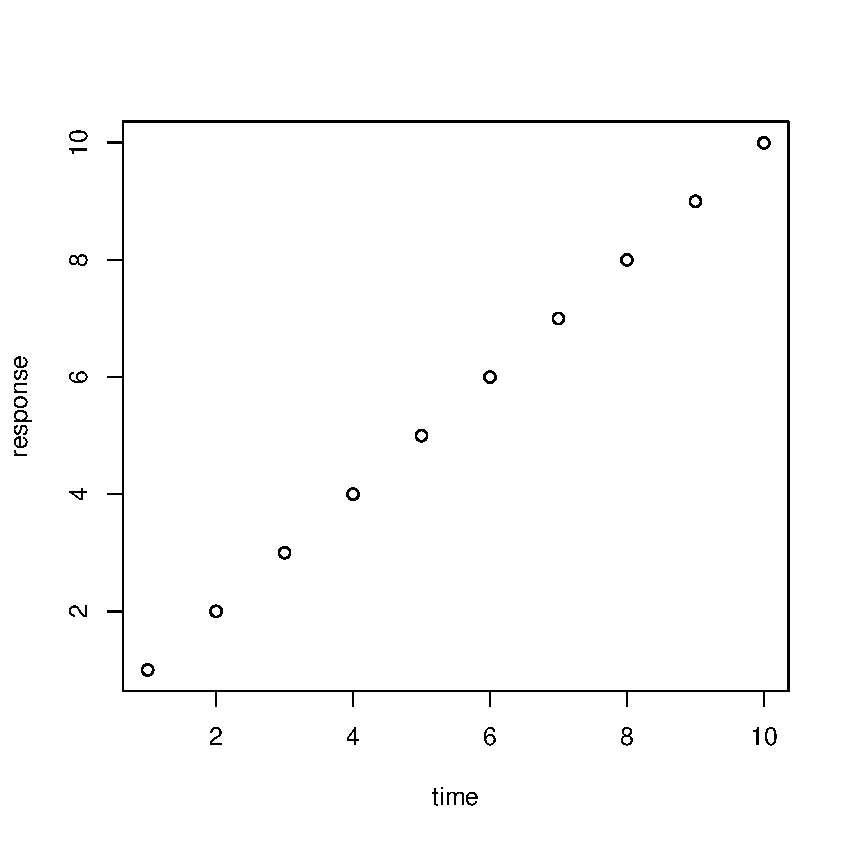
\includegraphics[width=3in]{fig1.pdf}
\end{center}
\caption{Caption of the figure. \label{fig:first}}
\end{figure}

\begin{table}[ht]
\caption{Caption of the table. \label{tab:tabone}}
\begin{center}
\begin{tabular}{rrrrr}
\toprule
one & two & three & four & five\\
\midrule
1.23 & 3.45 & 5.00 & 1.21 & 3.41 \\
1.23 & 3.45 & 5.00 & 1.21 & 3.42 \\
1.23 & 3.45 & 5.00 & 1.21 & 3.43 \\
\bottomrule
\end{tabular}
\end{center}
\end{table}

\section{Data and Methods}
\label{sec:meth}

\section{Results}
\label{sec:results}

\section{Conclusion}
\label{sec:conc}

\if0\blind
{
\section*{Acknowledgements}

The code and data for this paper are available at
\url{https://github.com/marysalvana/OpenSim-JCF-GP}.
} \fi

\bibliographystyle{agsm}
\bibliography{references}

\end{document}
